\documentclass{../../text-style}

\texttitle{Лекция 5: Проектирование пользовательских интерфейсов}

\begin{document}

\maketitle
\thispagestyle{empty}

\attribution{Тимофей Александрович Брыксин, бывш. доцент кафедры системного программирования СПбГУ}

\section{User Experience}

Современной компьютерной индустрии всего несколько десятков лет, а полноценно разнообразные гаджеты и интернет вошли в жизнь массового пользователя и вовсе не так давно. Сейчас человеко-машинное взаимодействие проникло практически во все сферы человеческой деятельности, и дальше будет проникать только всё сильнее. Интернет уже повсюду, у каждого ребёнка сейчас есть смартфон, и под это всё создаётся огромное количество самых разнообразных приложений\footnote{См., например, \url{http://goat-simulator.com/} (дата обращения: 12.03.2023).}. Всё это приводит к огромной конкуренции на рынке софта, а из неё естественным образом следует повышение качества приложений. Сейчас уже мало просто решить задачу, важно чем-то <<зацепить>> пользователя, сделать так, чтобы он вернулся, продолжил пользоваться вашим приложением или сайтом, посоветовал его друзьям и т.п. Сделать так, чтобы ваше приложение чем-то ему запомнилось, чтобы ему не хотелось больше пользоваться ничем другим. Всё это очевидным образом связано не только с функциональностью приложения, но и с look \& feel и даже с уровнем сервиса.

\begin{center}
    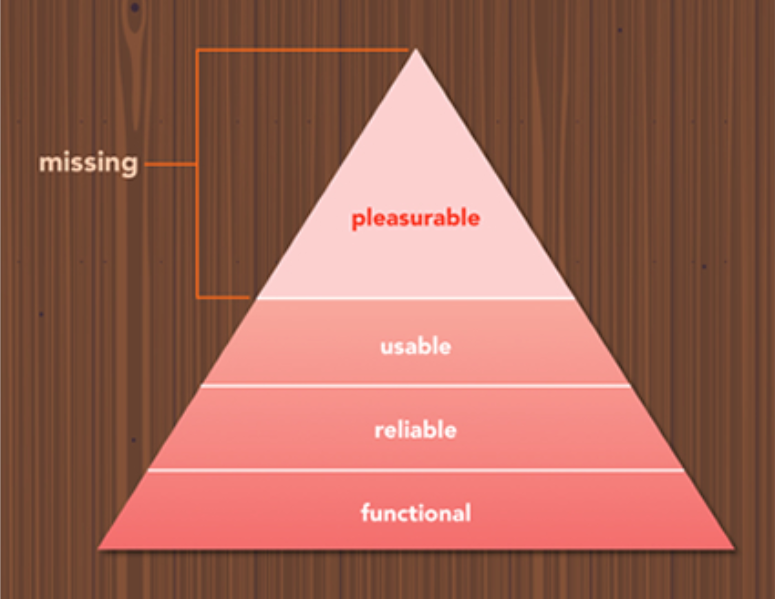
\includegraphics[width=0.6\textwidth]{uxPyramid.png}
\end{center}

Всё это привело к появлению термина User eXperience, UX (опыт пользователя или опыт взаимодействия), описывающего в целом восприятие и ответные действия пользователя, возникающие в результате использования продукции, системы или услуги. Опыт пользователя включает все эмоции, убеждения, предпочтения, ощущения, физические и психологические реакции пользователя, поведение и достижения, которые возникают до, во время и после использования системы. Опыт пользователя сочетает образ торговой марки, способ представления, функциональность, производительность системы, интерактивное поведение и вспомогательные возможности интерактивной системы, физическое и психологическое состояние пользователя, являющееся результатом предшествующего опыта, привычек, навыков и индивидуальности (ISO 9241-210).

\begin{center}
    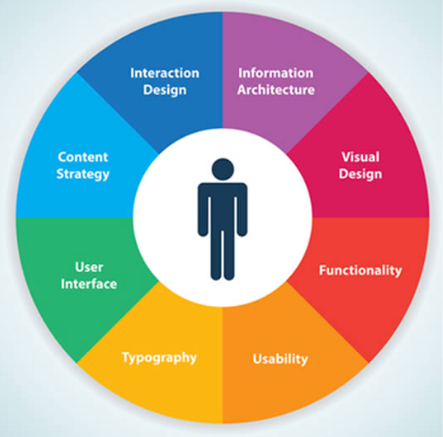
\includegraphics[width=0.5\textwidth]{uxComponents.png}
\end{center}

UX привлекает к себе очень много внимания, особенно когда это плохой опыт. Сейчас любят говорить о том, что хороший интерфейс незаметен для пользователя, люди пользуются им, не задумываясь. Но если UX спроектирован плохо, то это может вызвать много печали, раздражения или гнева, к тому же подобный опыт запоминается гораздо на дольше, чем хороший. Да, пока ещё в некоторых областях плохо спроектированные и реализованные приложения продолжают находить своих пользователей, но на западном массовом рынке сейчас такое долго не живёт\footnote{\url{http://usabilitygeek.com/business-structure-better-user-experience/} (дата обращения: 12.03.2023).}. Поэтому сейчас разработке каждого нового продукта (программного или более материального) предшествует (зачастую длительная) стадия анализа пользователей и проектирования взаимодействия с ними, иначе слишком велик риск сделать что-то ненужное или неюзабельное.

Область UX ещё очень молодая~--- определения, инструментарии и подходы ещё вовсю находится в процессе становления, но определённые наработки в этом направлении уже есть. UX design~--- это комплексное направление, которое включает в себя целую кучу всего\footnote{\url{https://github.com/envisprecisely/disciplines-of-ux} (дата обращения: 12.03.2023).}, включая аспекты психологии, антропологии, социологии, маркетинга, информатики и программирования, графического и промышленного дизайна, эргономики и многое другое. Изначально оно зародилось ещё в прошлом веке (или даже с появлением первых машин), однако взрывное развитие получило с ростом интернета, а затем и мобильных технологий. Когда ваш сайт или мобильное приложение могут быть одинаково доступны для пользователей по всему миру (ровно как и сайты/приложения конкурентов), вопросы их удобства использования, полезности и эффективности выходят на новый уровень. Поэтому большая часть публикаций на эту тему и и инструментов сейчас посвящено мобильной или веб-разработке, однако принципы применимы для весьма широкого круга продуктов.

Ещё стоит отметить, что для успешного проектирования UX о нём надо думать на всех стадиях разработки, начиная с предварительных исследований рынка и пользователей и проработки стратегии и заканчивая сопровождением и поддержкой. На картинке ниже показаны пять слоёв UX\footnote{\url{http://www.jjg.net/elements/pdf/elements_ch02.pdf} (дата обращения: 12.03.2023).} применительно к веб-сайтам\footnote{Кому лень читать больше одной страницы, альтернативная ссылка: \url{http://jjg.net/elements/pdf/elements.pdf} (дата обращения: 12.03.2023).}. 

\begin{center}
    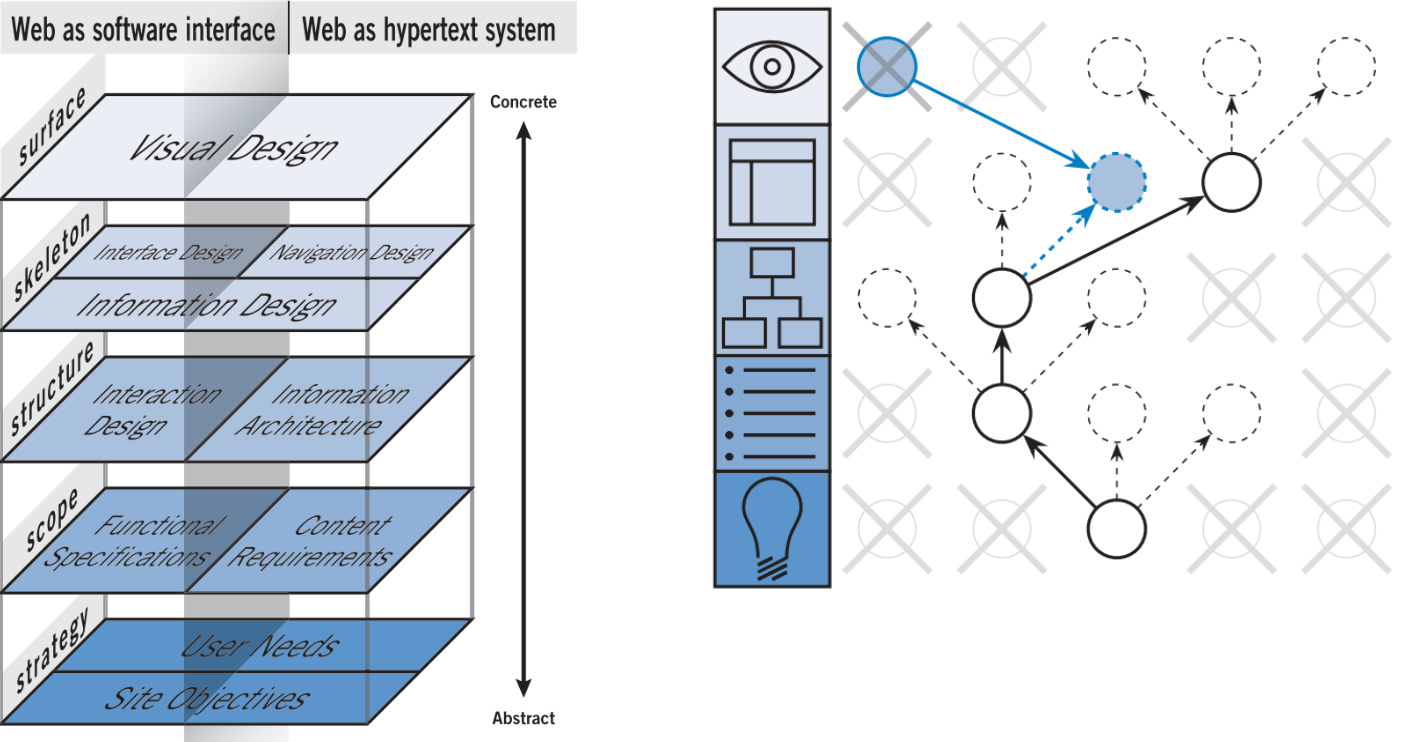
\includegraphics[width=0.8\textwidth]{uxLayers.png}
\end{center}

Каждый уровень зависит от соседних, и они должны быть в соответствии друг с другом. Если мы принимаем решения, которые противоречат другим уровням, цена разработки резко растёт, сроки пропускаются, а получившийся продукт вряд ли получится целостным. К тому же, решения, которые принимаются на более конкретных уровнях, вполне могут затрагивать решения на более абстрактных уровнях (например, при проектировании взаимодействия пришло более полное понимание о потребностях пользователей).

Ну и чтобы ответить на вопрос, зачем это всё инженерам-программистам, приведём вот такую картинку:

\begin{center}
    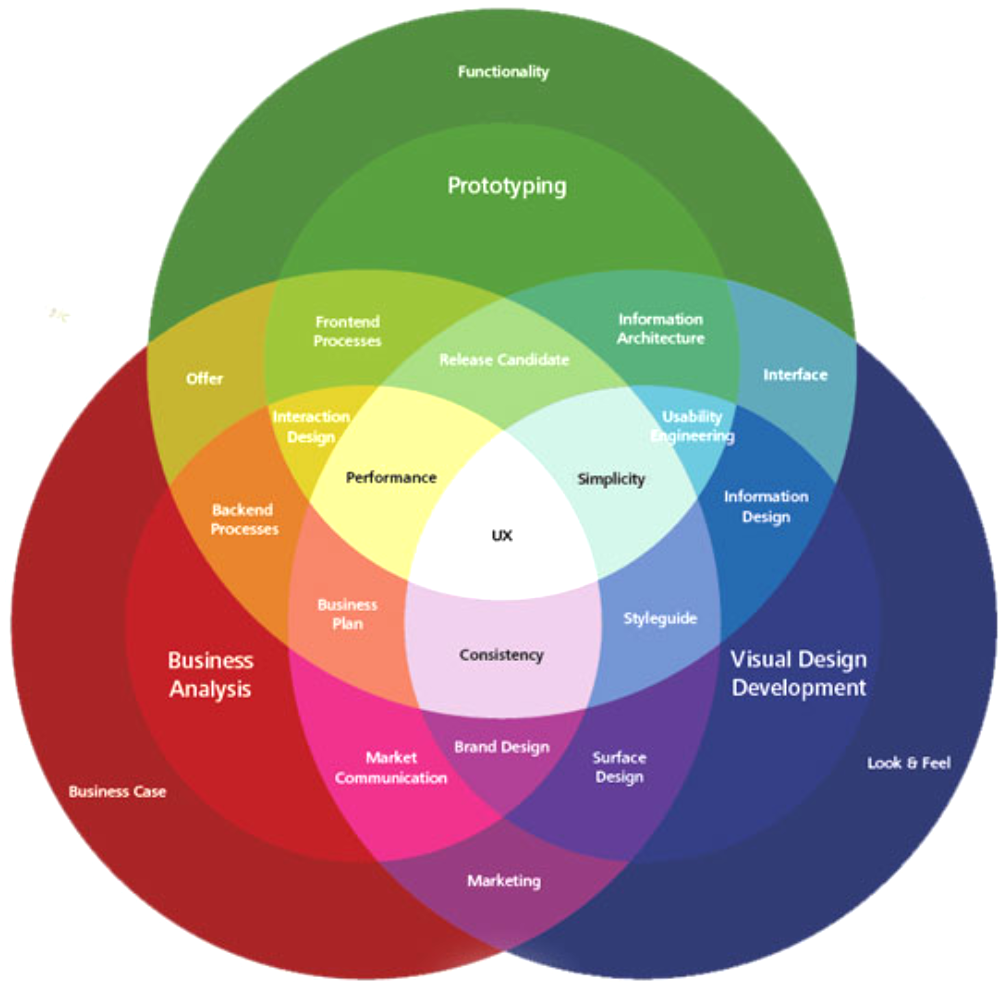
\includegraphics[width=0.8\textwidth]{uxDesignPractices.png}
\end{center}

Мы, как разработчики, отвечаем за зелёный кружок функциональности, и надо понимать, как жить и эффективно взаимодействовать с представителями остальных областей (бизнеса и маркетинга/дизайна). Понимание общих процессов разработки продукта делает нашу работу более осознанной. К тому же, как показывает практика, если адекватный технарь с хотя бы небольшим налётом гуманитарщины приходит в эту область, за счёт основательного и рационального мышления он там может добиться довольно многого.

Теперь поговорим о том, какие стадии проходит разработка UX продукта.

\section{Предварительные исследования}

Прежде, чем начать что-то делать, надо понять, что и для кого мы делаем.

\begin{itemize}
    \item Как продукт вписывается в контекст жизни пользователя? 
    \item Каковы основные цели людей в работе с продуктом? 
    \item Какие базовые задачи позволяют достигать целей? 
    \item Какой опыт люди находят привлекательным? Как он соотносится с продуктом?
    \item Какие проблемы встречаются у людей?
\end{itemize}

Собственно, тут бывает первичное исследование, включающее в себя непосредственное взаимодействие с людьми (интервью, полевое наблюдение, фокус-группы, метод тени, анкетирование, A/B тестирование и т.п.), и вторичное~--- анализ данных из открытых источников (почитать отзывы, новости в СМИ, анализ статистики и т.д.).

Также на ряд из поставленных вопросов можно ответить, составив одну или несколько из распространённых бизнес-моделей:

\begin{itemize}
    \item SWOT-анализ\footnote{\url{https://ru.wikipedia.org/wiki/SWOT-анализ} (дата обращения: 12.03.2023).};
    \item Business Model Canvas\footnote{\url{https://en.wikipedia.org/wiki/Business_Model_Canvas} (дата обращения: 12.03.2023).};
    \item Lean Canvas\footnote{\url{https://blog.leanstack.com/why-lean-canvas-vs-business-model-canvas/} (дата обращения: 12.03.2023).};
    \item Consumer Trend Canvas\footnote{\url{https://www.trendwatching.com/toolbox/consumer-trend-canvas} (дата обращения: 12.03.2023).};
\end{itemize}

Но это уже немного другая тема.

\section{Стратегия}

На этой стадии происходит определение того, что за продукт разрабатывается, для кого и что он в итоге будет собой представлять. По результатам этапа должно быть чётко сформулировано, что хочет аудитория (по результатам исследования потребностей пользователей) и бизнес-цели (с приоритетами).
Тут есть несколько вариантов.

\subsection{User-centered design}

В основе всего~--- пользователи\footnote{\url{https://en.wikipedia.org/wiki/User-centered_design} (дата обращения: 12.03.2023).}, всё строится вокруг их потребностей и целей, которые учитываются с самого начала и включены в полный жизненный цикл продукта:

\begin{center}
    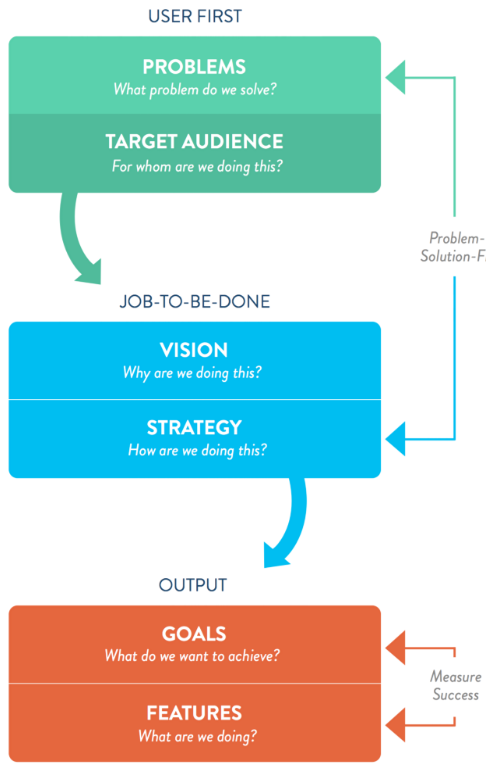
\includegraphics[width=0.4\textwidth]{userCenteredDesignProcess.png}
\end{center}

Полезно заполнять карточки примерно таких видов для всеобщего понимания стратегии:

\begin{center}
    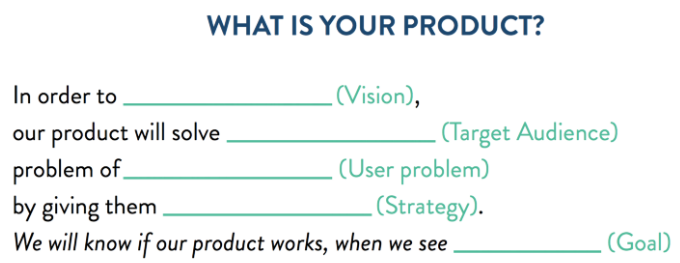
\includegraphics[width=0.6\textwidth]{productCard.png}
\end{center}

Для \textcolor{green}{(целевых пользователей)}, которым нужно \textcolor{green}{(потребность)}, \textcolor{green}{(Название продукта)}~--- это \textcolor{green}{(рыночная категория)}, который \textcolor{green}{(одно ключевое преимущество)}.

\vspace{5mm}

В отличие от \textcolor{green}{(конкуренты)}, \textcolor{green}{(Название продукта)} \textcolor{green}{(уникальное отличие)}.

Пример:

Для частных строительных бригад, которым нужно отслеживать доступность дороги на строительной площадке, \textcolor{green}{(Название продукта)} это коммуникационный инструмент, который сообщает бригаде, когда дорога будет закрыта. В отличие от текущей бумажной системы, \textcolor{green}{(Название продукта)}~--- это веб сервис, доступный всем работникам в любое время в любом месте.

\paragraph{Персонажи}

Чтобы понять жизнь потенциальных пользователей, их мотивацию и среду обитания, проводятся наблюдения, интервью и другие исследования, в результате появляются достаточно объемные данные, необходимые для проектирования успешного продукта. Одним из путей использования этих данных в дальнейшем является создание на их основе описательных моделей пользователей. Такие модели пользователей принято называть персонажами. Каждый персонаж строится на основе мотивации и поведенческих шаблонов реальных людей, которые участвовали в наблюдениях и интервью, и выступает в роли представителя значимого подмножества целевой аудитории в процессе проектирования. Персонажи помогают понять цели пользователей в конкретных ситуациях, а также преобразовать данные о пользователях в проектные решения.

Использование персонажей позволяет выделить и подробно рассмотреть основные типы пользователей, оценить их потребности, выбрать группу наиболее важных пользователей и в дальнейшем ориентироваться на них при проектировании функциональности и поведения продукта, при этом стараясь не причинять существенных неудобств остальным пользователям.

Персонажи~--- это модели пользователей, представленные в виде отдельных, конкретных людей. Успех персонажей как моделей пользователей во многом определяется тем, что персонажи олицетворяют личности и часто вызывают сопереживание проектировщиков по отношению к людям, ради которых выполнялось проектирование. Персонажи не только помогают проектировщикам найти решения, лучше отвечающие действительным потребностям пользователей, но и делают эти решения более обоснованными в глазах заинтересованных в реализации лиц. Если персонажи разработаны тщательно и корректно, заинтересованные лица и инженеры начинают думать о них как о настоящих пользователях и проявляют гораздо больший интерес к созданию продукта, который станет источником положительного опыта для этих персонажей.

Обычно целевая аудитория продукта группируется в 3-4 основных персонажа. Идеально 2-3, больше 5~--- это уже проблема, в этом случае интерфейс системы будет сильно перегружен, чтобы одновременно удовлетворить всем группам пользователей, либо какие-то группы пользователей пострадают. В этом случае рекомендуется разбить систему на две.

Персонажи позволяют решать основные проблемы, возникающие при разработке продукта.

\begin{itemize}
    \item Проблема пластилинового пользователя заключается в возможности подстройки представления о пользователе под мнения и предположения разработчиков, тогда как требуется решение, удовлетворяющее потребности реальных пользователей.
    \item Проблема проектирования под себя, когда пользователь продукта наделяется качествами проектировщика или разработчика. Персонажи содержат конкретные требования, основанные на целях реальных пользователей, их способностях и контексте использования продукта. Использование персонажей в процессе проектирования не позволяет слишком вольно обращаться с понятием <<пользователь>>.
    \item Проектирование в расчете на исключительные ситуации. Персонажи дают возможность проверять решения на соответствие реальности, позволяют четко назначать приоритеты различным функциям.
\end{itemize}

Для каждого типа персонажа составляется документ-описание в произвольном формате. Например, они могут выглядеть так:

\begin{center}
    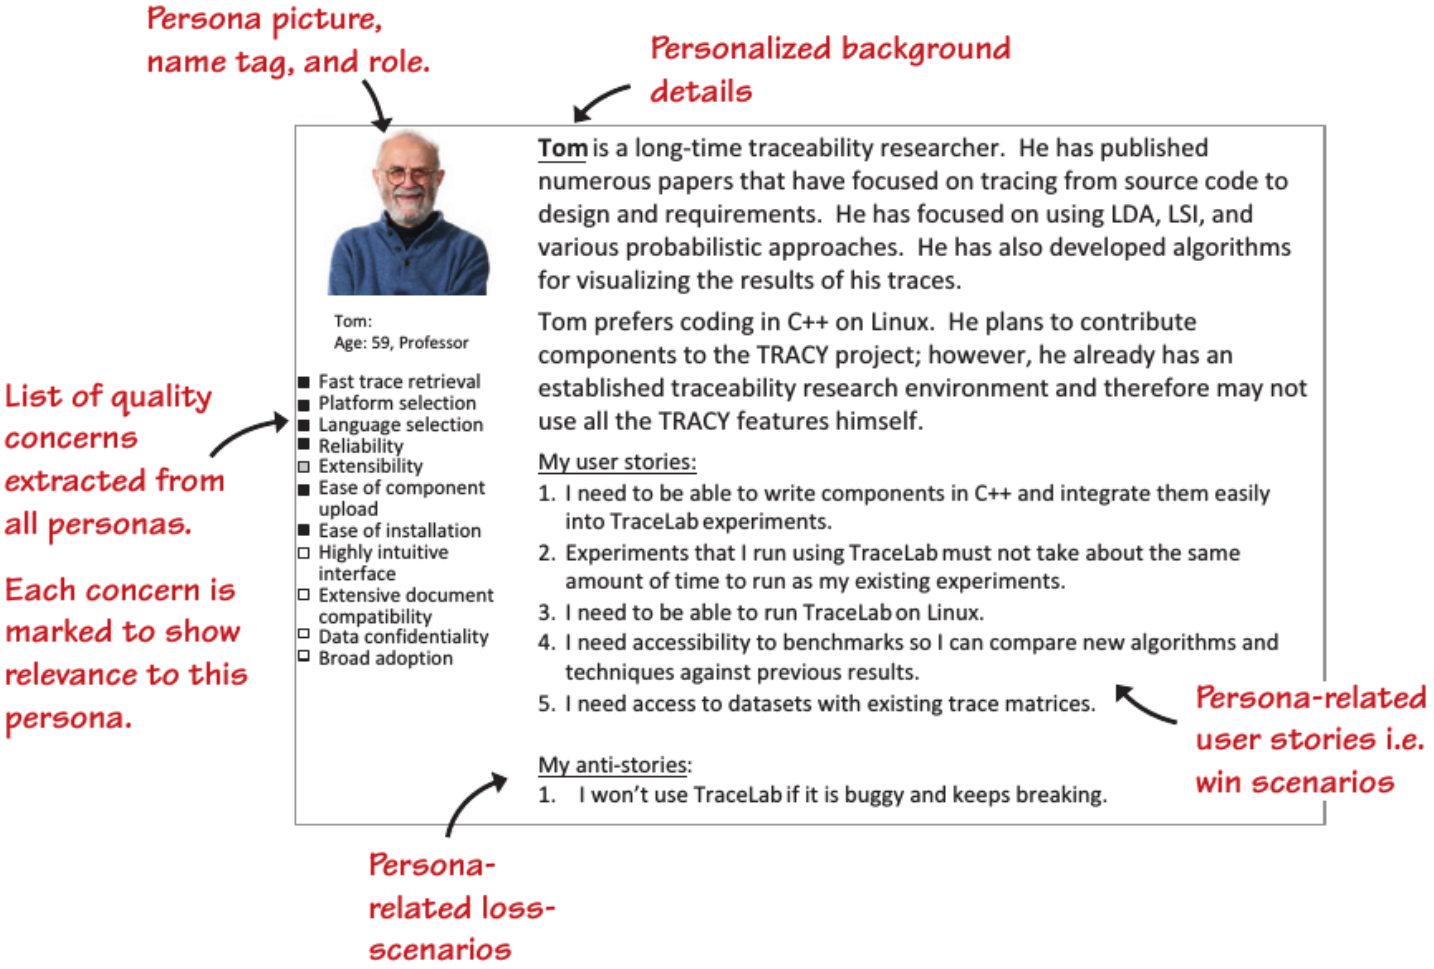
\includegraphics[width=0.9\textwidth]{tom.png}
\end{center}

или так:

\begin{center}
    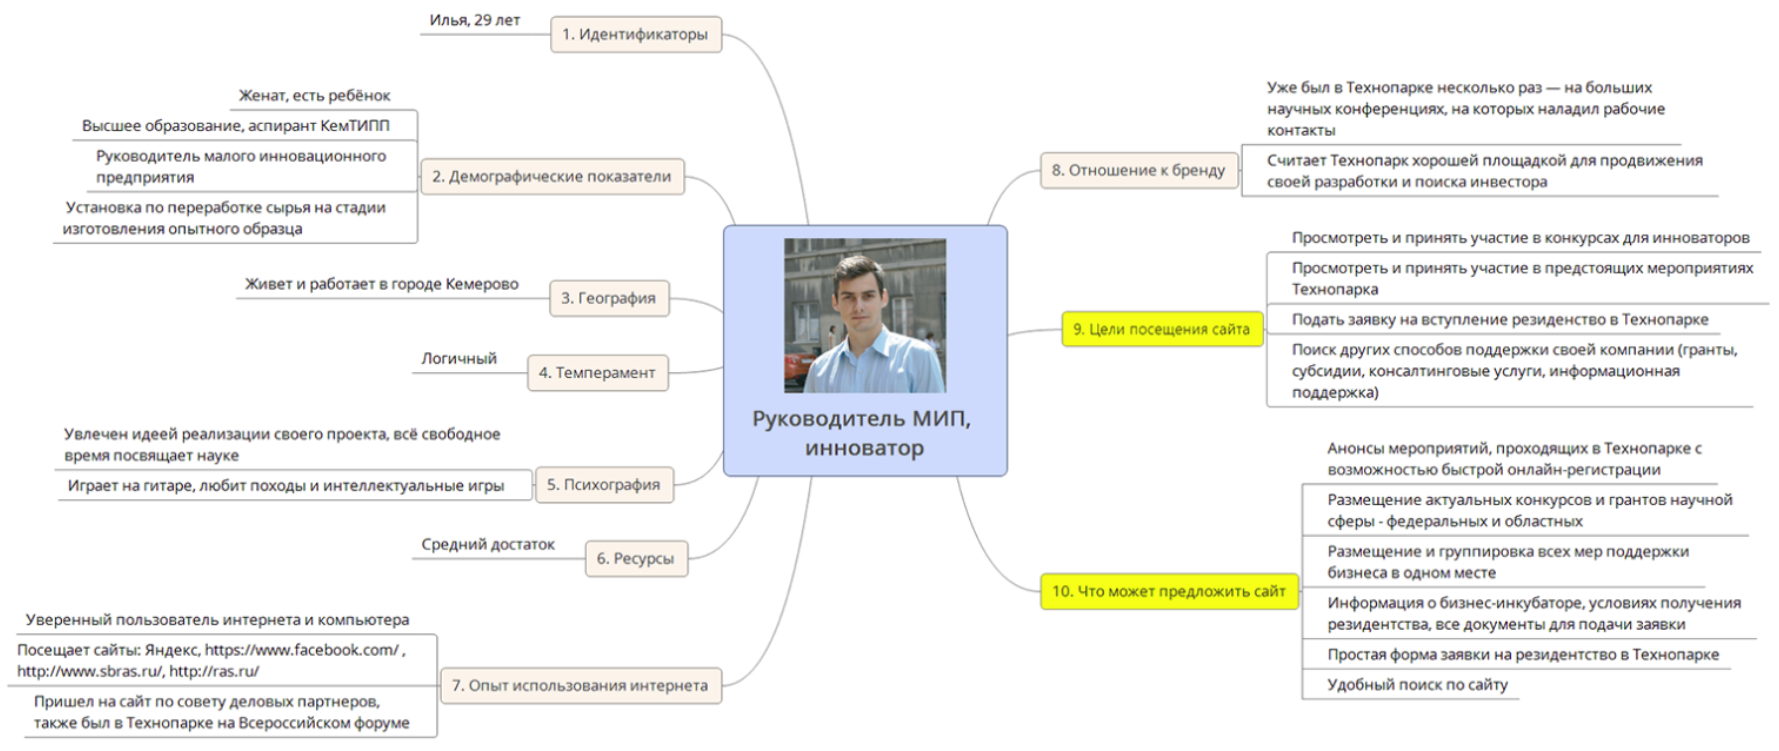
\includegraphics[width=0.9\textwidth]{ilya.png}
\end{center}

Про то, как организовать процесс построения персонажей, можно прочитать тут: \url{https://uxexperience.net/useful/artefakty-persona} (дата обращения: 12.03.2023). А про то, сколько времени может занимать эта работа~--- тут: \url{https://www.nngroup.com/articles/persona-budgets/} (дата обращения: 12.03.2023).

В книге Agile Software Architecture\footnote{\url{https://www.oreilly.com/library/view/agile-software-architecture/9780124077720/} (дата обращения: 12.03.2023).} (глава 4) также описывается подход, при котором созданные персонажи использовались и для анализа архитектурных решений, оценки рисков и т.п. Так что с точки зрения разработчика это совсем не такая бесполезная работа, как может показаться поначалу.

\paragraph{Сценарии}

Информацию о пользователях и их целях, полученную из описаний персонажей, можно использовать для создания сценариев, описывающих идеальное для пользователя взаимодействие с продуктом. По сути создаются повествования о том, как будет использоваться продукт.

Рассмотрим три типа сценариев, основанных на персонажах и используемых на различных этапах проектирования.

\begin{itemize}
    \item Контекстные сценарии создаются до начала проектирования, пишутся с точки зрения персонажа, сосредоточены на человеческих действиях, впечатлениях и желаниях, позволяют определить, как продукт может наилучшим образом послужить потребностям персонажей.
    \item Сценарии ключевого пути появляются в результате пересмотра контекстных сценариев путем добавления к ним более подробных описаний взаимодействия пользователя с продуктом.
    \item Проверочные сценарии используются для тестирования проектных решений в различных ситуациях, обычно имеют форму набора вопросов: <<а что, если...?>>, касающихся предложенных решений.
\end{itemize}

Сценариев может быть много (особенно если много разных персонажей), в этом случае надо выбрать самый популярный сценарий и делать дизайн под него. Или как-то понимать, в рамках какого сценария пользователь пришёл к вам в продукт, и адаптировать внешний вид соответственно (если это применимо). Например, можно показывать разные страницы регистрации для разных типов пользователей. Если так сделать не получается~--- найти наименьший общий знаменатель: изначально должна быть видна только основная функциональность, доступная для всех.

На этом этапе можно создавать модели сценариев использования, про которые мы говорили ранее. Кроме этого в больших проектах, а также при создании принципиально нового продукта могут использовать раскадровки (storyboarding, см. далее).

\subsection{Activity-centred design}

Подход, который ориентируется не на пользователей и их потребности, а на действия, которые пользователь совершает для решения задачи, и которые создаваемые продукты должны поддерживать. Подход рассматривает систему в целом без расчёта на каких-то конкретных пользователей.

Большая часть объектов современного мира разрабатывалась без какого-либо учёта персонажей и сценариев, и люди как-то водят автомобили, пользуются сложными приборами, играют на музыкальных инструментах, отмеряют время в странных системах счисления (7-, 12-, 60-ричных), хотя что-то из этого может быть довольно сложно, и им приходится долго учиться. А всё потому, что эти инструменты идеально заточены для решения тех задач, ради которых люди их используют, а люди обладают очень большими способностями к обучению. 

User-based проектирование может быть даже вредно в случае, если у продукта слишком много разных групп пользователей, подстроиться под всех не получится, всё равно кто-то останется в обиде. К тому же, персонажи со временем могут меняться (с получением опыта или просто ввиду трендов в обществе). К тому же, как твердили Форд и Джобс, пользователи сами часто не знают, чего хотят, и задача проектировщика узнать это за них и сделать такой продукт. Но в этом случае проектировщик должен быть реально крутой, и очень многое зависит от того, насколько правильным окажется его видение продукта и его использования.

Разумеется, никто не говорит, что надо забить на пользователей и делать всё, как нам захочется. Данный подход всё так же анализирует поведение пользователей, однако тут скорее идёт анализ того, что пользователь делает с инструментом/продуктом, и насколько это приближает его к решению изначальной задачи\footnote{Про всё это поподробнее можно почитать по ссылкам \url{http://jnd.org/dn.mss/human-centered_design_considered_harmful.html} (дата обращения: 12.03.2023) и \url{https://medium.com/@collabject/stop-designing-for-users-9c5e582b3ec8} (дата обращения: 12.03.2023).}.

\subsection{Data-driven design}

Проектирование, основанное на данных, очень хорошо применять, собственно, когда есть какие-то данные о продукте. Анализируя данные, мы можем принимать более адекватные решения при проектировании системы. Это может быть публичная или инсайдерская информация о конкурентах, либо данные по уже созданному прототипу или даже работающей системе, если делаем редизайн или пытаемся что-то оптимизировать в продукте. Также в качестве исходных данных можно использовать публикуемые маркетинговые исследования и аналитические статьи.

Например, в статье <<Data-Driven Design In The Real World>>\footnote{\url{https://www.smashingmagazine.com/2013/09/data-driven-design-in-the-real-world/} (дата обращения: 12.03.2023).} подробно расписывается, как товарищи проанализировали данные по посещениям пользователями страниц их сайта, спроектировали новую страницу регистрации, получилось плохо, проанализировали данные ещё раз, придумали новую гипотезу, спроектировали новую страницу, и всё у них получилось.

\section{Информационная структура}

Под информационной архитектурой понимают структуру информационной системы, интерактивных сервисов и пользовательского взаимодействия с ними, приводящего к решению поставленной задачи. Информационная структура разрабатывается часто на основе пользовательских сценариев и позволяет определить ключевые точки системы, места принятия решений при выполнении тех или иных действий.

Выделяют несколько классических типов информационной архитектуры.

\begin{itemize}
    \item \textbf{Категории.} Это самый распространенный вид информационной архитектуры, содержимое упорядочивается по его типу. Например, для интернет-магазина одежды пользователи ожидают увидеть категории Мужчины, Женщины, Дети, Распродажа и т.п.
    \item \textbf{Задачи.} Структура основывается на задачах, которые пользователю нужно решить. Если проектируется приложение для банка, то задачи могут быть примерно такие: Вклады, Займы, Инвестиции, Помощь, Открытие счета. Тут важно не ошибиться с требованиями к пользователю: если у него не будет достаточной квалификации, он может просто не разобраться в этих задачах и потеряться.
    \item \textbf{Поиск.} Данный тип подходит для приложений или сайтов, которые состоят из содержимого, создаваемого самими пользователями. Например, если бы у YouTube были только категории (смешное, грустное, реклама, фильмы и др.), пользоваться сайтом было бы сложно и много усилий уходило бы на поддержание категорий в порядке.
    \item \textbf{Время.} Пример такого типа архитектуры~--- почтовый ящик, где сообщения отображаются по мере доставки. Это и есть дизайн, построенный на времени. В случае с веб-сайтом, это бы выглядело как страницы типа: <<актуально прямо сейчас>>, <<в архиве>>, <<почитать позже>>, <<новинки>> и т.п. Примеры такого временного дизайна~--- это Reddit или новостная лента в соцсетях.
    \item \textbf{Люди.} Любая соцсеть~--- это информационная архитектура, построенная на людях. Дизайн вращается вокруг конкретного человека и его отношений с другими людьми. А вот внутри каждого профиля обычно используется организация информации в систему категорий (фотографии, друзья, места).
\end{itemize}

Для визуализации информационной структуры в самых простых случаях может использоваться просто перечисление страниц сайта или экранов приложения с указанием зависимостей или переходов (карта сайта или приложения):

\begin{center}
    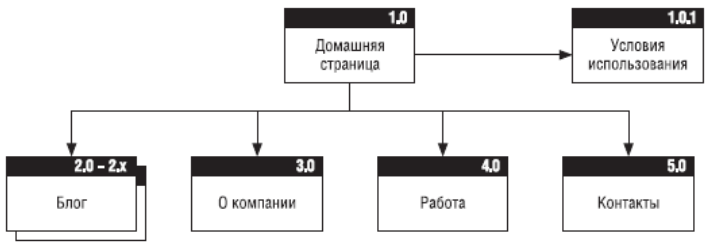
\includegraphics[width=0.8\textwidth]{informationStructureSmall.png}
\end{center}

Пример из реальной жизни для мобильного приложения:

\begin{center}
    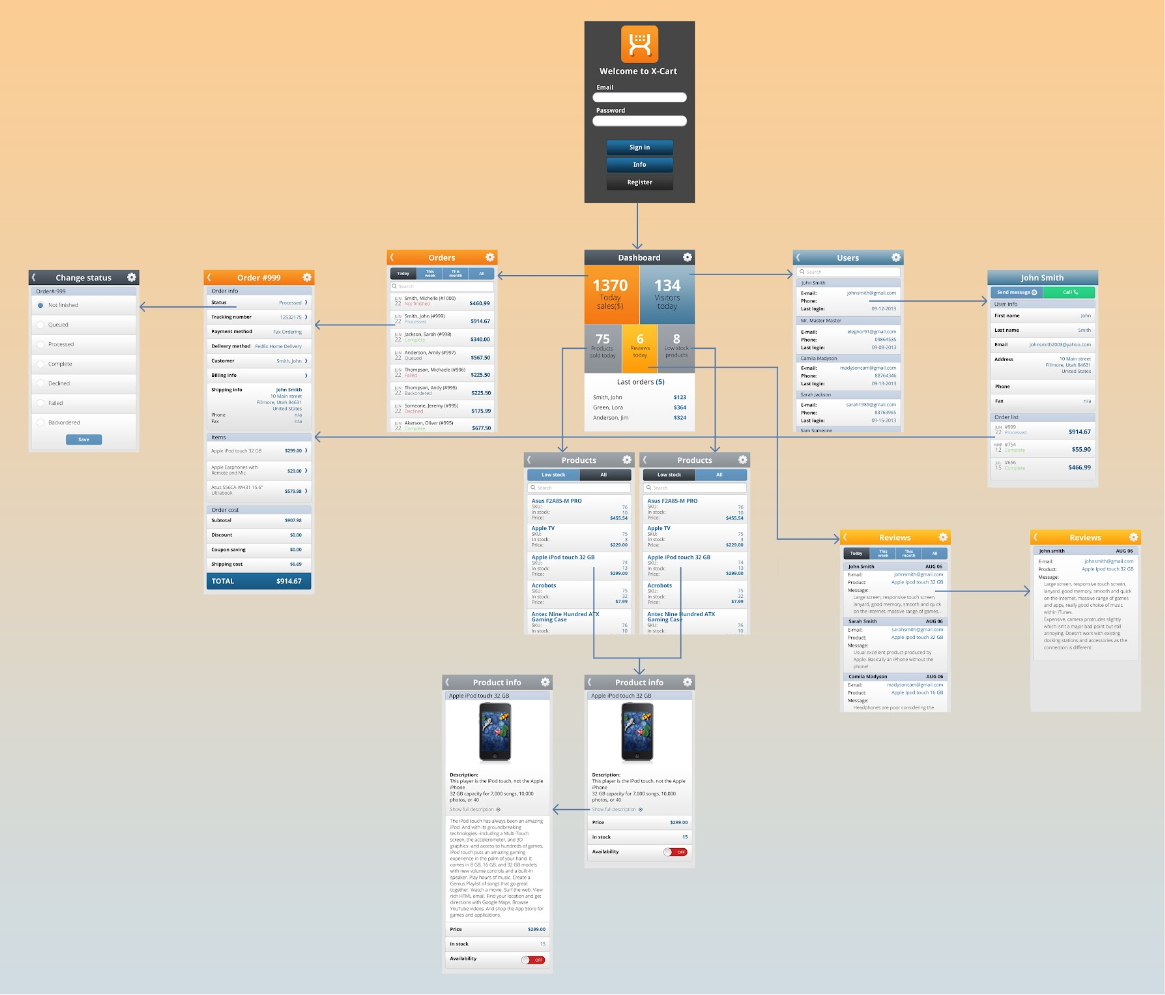
\includegraphics[width=0.95\textwidth]{screenMap.png}
\end{center}

В случае activity-centered design полезной будет предварительная схема с задачами по каждому экрану:

\begin{center}
    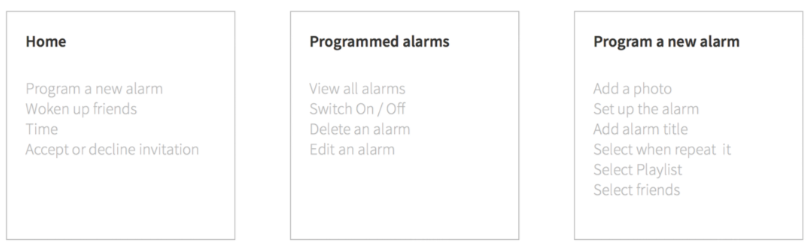
\includegraphics[width=0.8\textwidth]{screenTasks.png}
\end{center}

Также для этих целей подойдёт mindmap, UML или любая другая диаграмма, подходящая для отображения пользовательских сценариев:

\begin{center}
    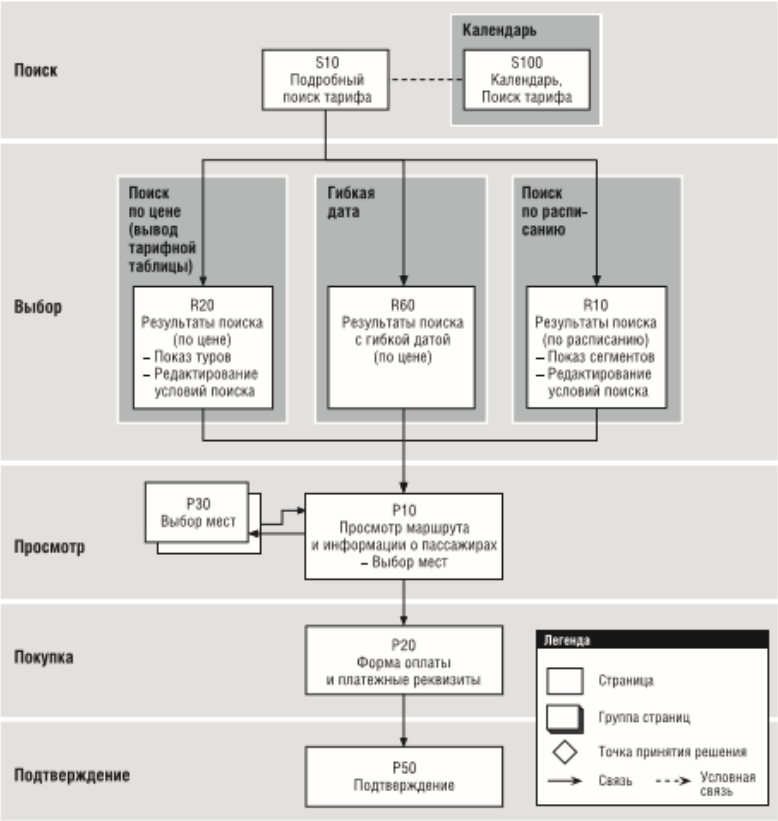
\includegraphics[width=0.65\textwidth]{userScenario.png}
\end{center}

Дополнительно бывает полезно выписать в обычной таблице все возможные страницы сайта. Так, например, можно первично спроектировать их адреса и заголовки:

\begin{center}
    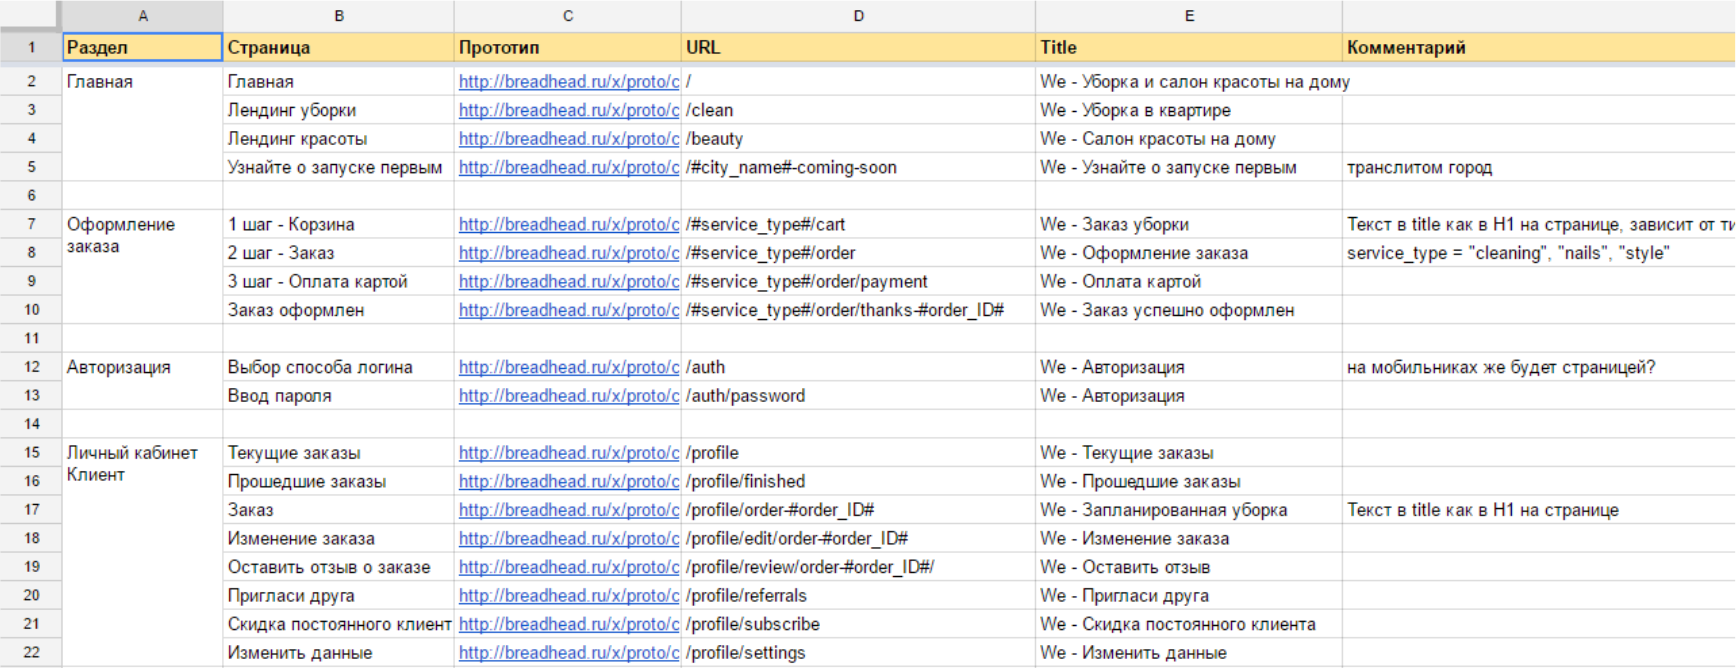
\includegraphics[width=\textwidth]{tableView1.png}
\end{center}

Или даже сделать первую оценку по трудоёмкости разработки:

\begin{center}
    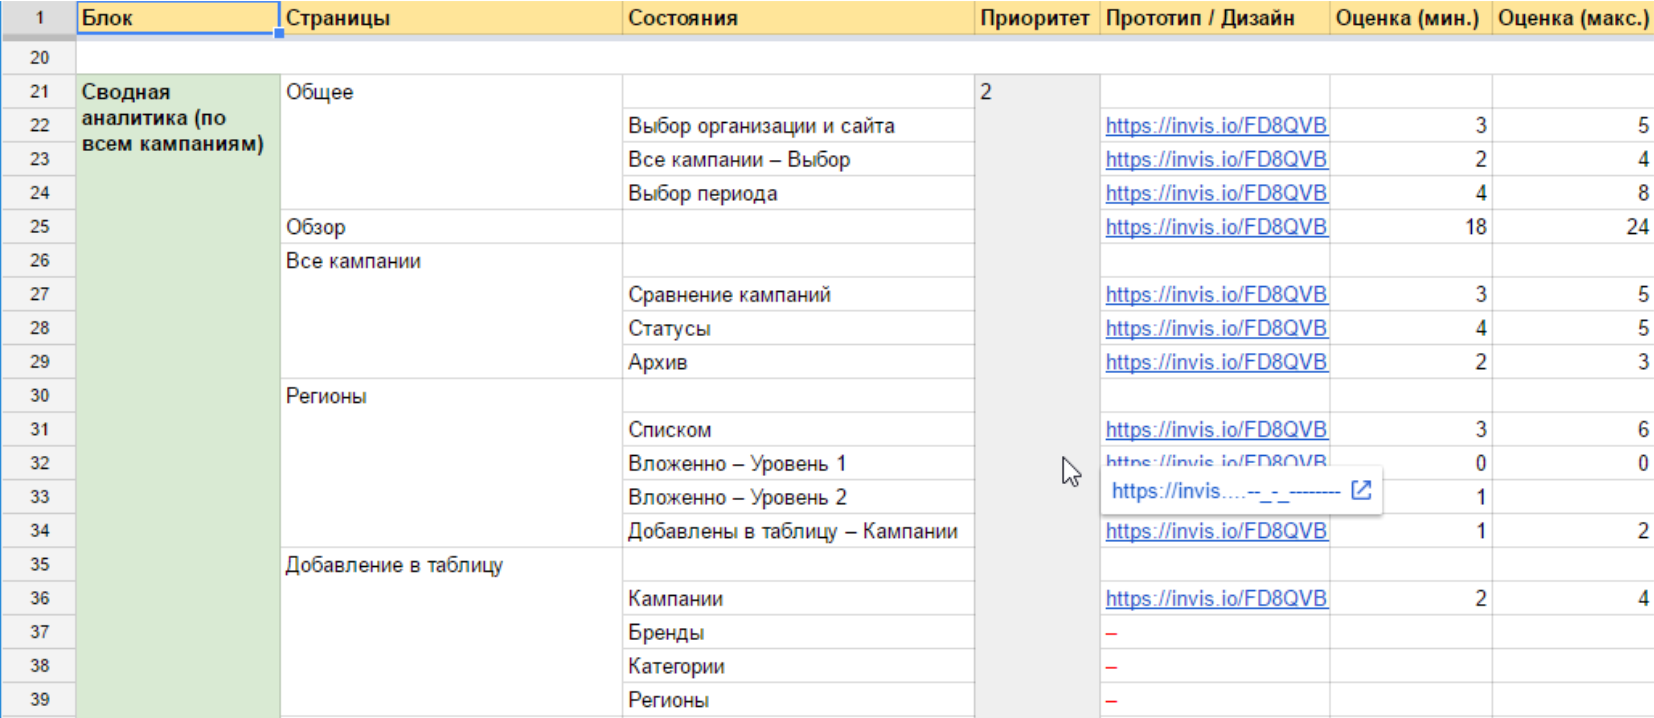
\includegraphics[width=\textwidth]{tableView2.png}
\end{center}

В более сложных случаях проектирования UX (особенно при взаимодействии нескольких приложений или сервисов) используется практика построения карты путешествий клиента (customer journey maps). Эти карты описывают полный путь пользователя во взаимодействии с продуктом (или продуктами, если во взаимодействие их вовлечено сразу несколько), выделяются ключевые точки, описывается эмоциональное состояние пользователей, их пожелания, потребности, факторы принятия решений и многое другое. 

\begin{center}
    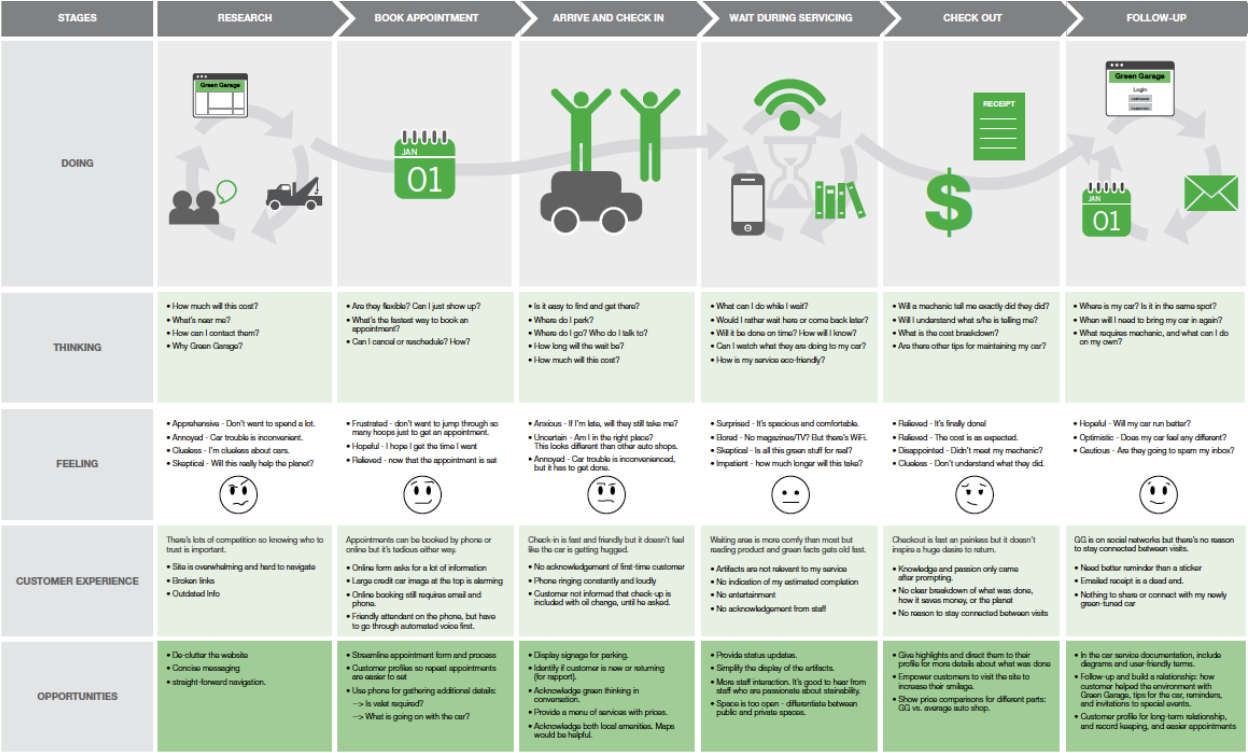
\includegraphics[width=\textwidth]{customerJourneyMaps.png}
\end{center}

Всё это в целом дальше можно анализировать, искать узкие места во взаимодействии или обслуживании, сравнивать с количественными данными при эксплуатации системы и т.п.\footnote{Подробнее с примерами можно почитать, например, тут: \url{https://medium.com/@copylove/customer-journey-map-8a5ac61d6b5e} (дата обращения: 12.03.2023).}

\section{Прототипирование}

Когда стало хотя бы примерно понятно, что же, собственно, представляет собой продукт, самое время перейти к прототипированию его интерфейса. Для поддержки этого процесса есть целая куча практик разной степени формальности и детализации:

\begin{center}
    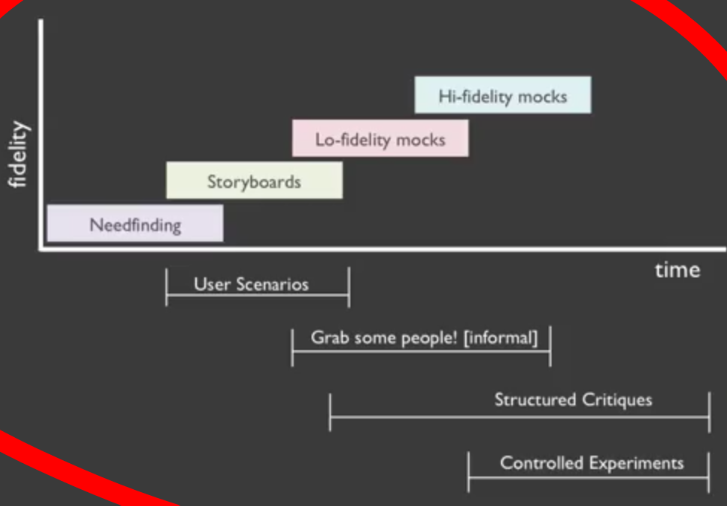
\includegraphics[width=0.7\textwidth]{prototypingTechniques.png}
\end{center}

Рассмотрим самые популярные из них.

\subsection{Storytelling}

Самый неформальный и простой подход: пользовательские сценарии описываются словами в виде литературных историй. Люди любят хорошие истории, к ним можно возвращаться во время проектирования интерфейса, на них можно основывать тестирование и т.п. Истории помогают разработчикам понять пользователей, узнать их цели, помогают аналитикам представить результаты исследований, проектировщикам продемонстрировать варианты дизайна.

\subsection{Storyboarding}

Раскадровки (или сториборды) активно используются в киноиндустрии, и там они доведены до такого совершенства, что ещё до начала съёмок чётко распределено, что будет происходить в каждую секунду полуторачасового фильма. Стоимость времени реальных съёмок настолько велика, что на ходу что-то менять и перепроектировать никто в здравом уме никогда не возьмётся. Поэтому в фильмах все сцены заранее прорисовываются и утверждаются, иногда даже на них накладывают музыку и прокручивают, чтобы ещё на первых стадиях оценить зрелищность и сюжет фильма. Сториборды, сохраняя название и форму, как в киноиндустрии, при проектировании интерфейсов выполняют немного другие задачи.

Некоторые эксперты предлагают их использовать внутри команды, чтобы формировать общее видение для всех членов рабочей группы. Другие советуют использовать их для презентации заказчикам своих решений. Периодически сториборды выступают ещё и как этап проектирования где-то между формированием персонажей и рисованием первого прототипа системы.

Понятно, что сториборды для всех трех задач будут разными. В любом случае, сториборд должен отвечать на вопросы (неважно, клиента или ваших коллег):

\begin{itemize}
    \item Кто ваш персонаж?
    \item Какую потребность удовлетворяет система?
    \item Какая задача должна быть выполнена?
    \item Что приводит пользователя к использованию вашей системы?
    \item В каких условиях оно выполняется?
    \item Какова последовательность действий?
    \item Какие у пользователей есть возможности?
\end{itemize}

Например, ниже приведён пример сториборда для одного из сценариев использования программы с рецептами печенья. Каждый сториборд должен показывать проблему пользователя (первые четыре квадрата), решение (пятый квадрат) и выгоду для бизнеса (шестой квадрат). Здесь это распространение приложения между пользователями и высокие оценки в рейтинге. Нет смысла показывать клиенту, как мальчик съел печеньку, его (клиента) цель~--- продать приложение или продать рекламу в популярном приложении.

\begin{center}
    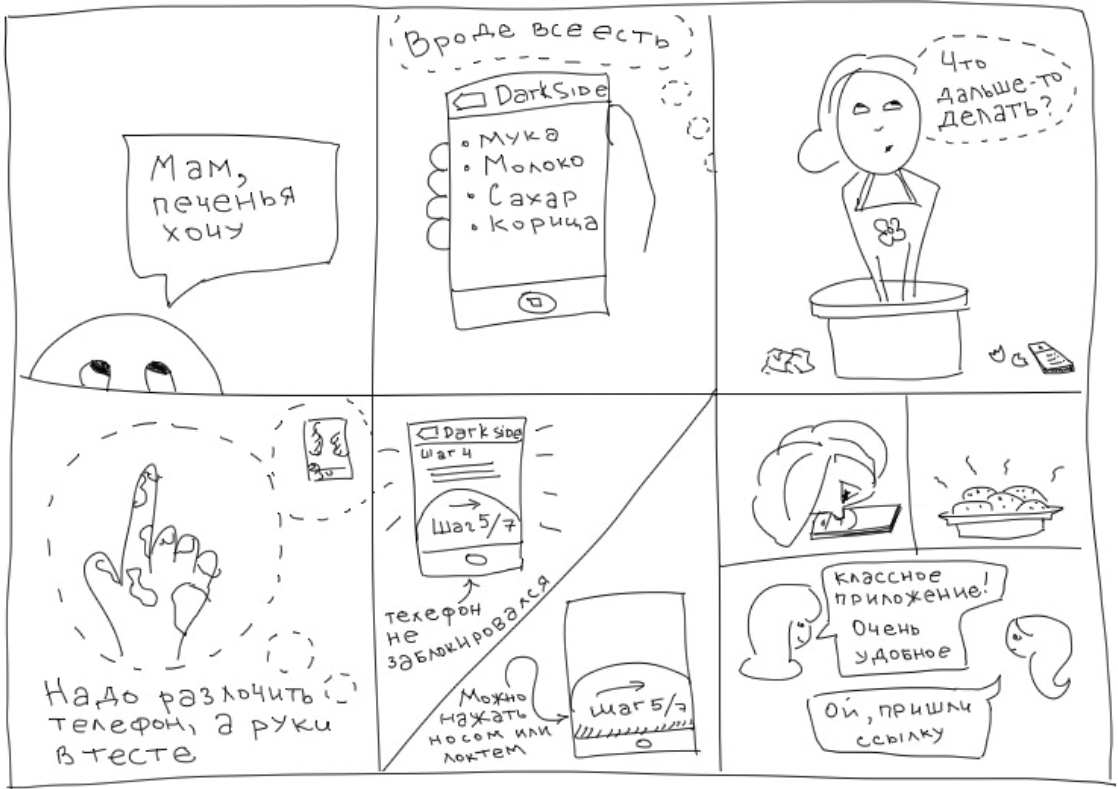
\includegraphics[width=0.7\textwidth]{storyboardingExample.png}
\end{center}

Как рисовать, не особо важно, главное, чтобы смысл передавался. Для тех, кто не умеет рисовать и не хочет позориться, есть всякие инструменты типа \url{https://boords.com/} или \url{https://www.storyboardthat.com}, которые позволяют это дело автоматизировать\footnote{Как обычно, подробнее можно много где почитать: 
\begin{itemize}
    \item \url{http://www.uxmatters.com/mt/archives/2011/11/using-storyboards-and-sentiment-charts-to-quantify-customer-experience.php} (дата обращения: 12.03.2023).
    \item \url{https://uxknowledgebase.com/storyboarding-part-1-7d020f468420} (дата обращения: 12.03.2023).
\end{itemize}.}.

\subsection{Бумажные прототипы}

Смысл бумажных прототипов в том, чтобы минимальными усилиями из подручных средств сделать некий макет приложения ещё до создания каких-либо прототипов и попробовать <<использовать>> этот макет в рамках определённых сценариев.

Можно снять покадровое видео\footnote{\url{https://speckyboy.com/10-effective-video-examples-of-paper-prototyping/} (дата обращения: 12.03.2023).} или записать полноценный ход процесса\footnote{\url{https://www.youtube.com/watch?time_continue=74&v=V8LNDqMIapY} (дата обращения: 12.03.2023).}, самое важное тут~--- попробовать максимально реалистично (насколько это возможно) проговаривать основные действия пользователя и их мотивацию. При наличии хорошо проработанных персонажей и сценариев это не должно быть очень сложно. Достоинства подхода~--- результат можно получить очень быстро, достаточно по сути только телефона или камеры. Уровень проработанности не так важен, можно рисовать на бумаге ручкой, использовать специальные трафареты или просто клеить стикеры на телефон.

Этот подход очень хорошо подходит для понимания MVP\footnote{\url{https://en.wikipedia.org/wiki/Minimum_viable_product} (дата обращения: 12.03.2023).} и проработки основ взаимодействия пользователя с продуктом (например, можно внезапно обнаружить, что забыли что-то важное).

\subsection{Bodystorming}

Ещё один вариант дешёво и сердито замоделировать работу приложения или опробовать продукт~--- Bodystorming. По сути~--- разыгрывание сценки между группой людей. Один человек (чаще всего член команды) изображает систему, другие (поначалу лучше друзья, а потом возможно даже совсем посторонние по отношению к проекту люди)~--- пользователей. Оператор вслух комментирует происходящее с точки зрения приложения, <<пользователи>>~--- с точки зрения пользователей.

Со стороны может выглядеть как полная наркомания\footnote{См., например, \url{https://www.youtube.com/watch?v=AoWAnY2La5k} (дата обращения: 12.03.2023).}, однако опять же позволяет очень быстро и дёшево проверить основные сценарии работы и что пользователи вообще думают об идее проекта. Очень хорошо сочетается с бумажными прототипами.

\subsection{Wireframe (макеты)}

Wireframe~--- это набор схематичных макетов экранов приложения или страниц сайта. Основная цель~--- высокоуровнево спроектировать внешний вид экранов и показать компоновку графических элементов на них. Макеты обычно создаёт проектировщик интерфейсов, и у них есть несколько основных применений.

\begin{itemize}
    \item Их можно использовать как техническое задание графическому дизайнеру. При отрисовке макетов страниц дизайнер должен не забыть все указанные в макетах элементы и учитывать расставленные акценты.
    \item Эти же самые макеты являются и техническим заданием разработчикам, которые руководствуются ими при создании функционального прототипа системы (уже работающая система, к которой еще не <<прикручен>> дизайн).
    \item Макеты также можно использовать для демонстрации инвесторам и потенциальным пользователям. Система может быть показана заинтересованным лицам уже через несколько недель после начала работ, и она уже не выглядит так потешно, как бумажный прототип.
\end{itemize}

В самом простом варианте он превращается в диаграмму зонирования (reference zone), на которой показаны только блоки:

\begin{center}
    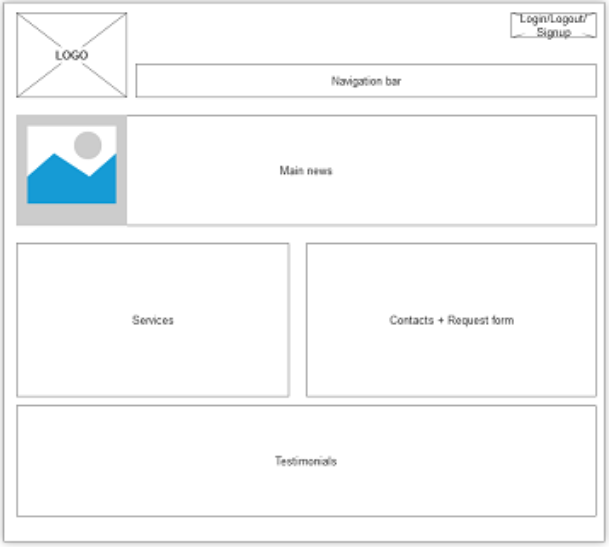
\includegraphics[width=0.6\textwidth]{wireframe.png}
\end{center}

В более продвинутом варианте, например, страница курса с точки зрения пользователя-студента на сайте по изучению английского языка может выглядеть как-то так:

\begin{center}
    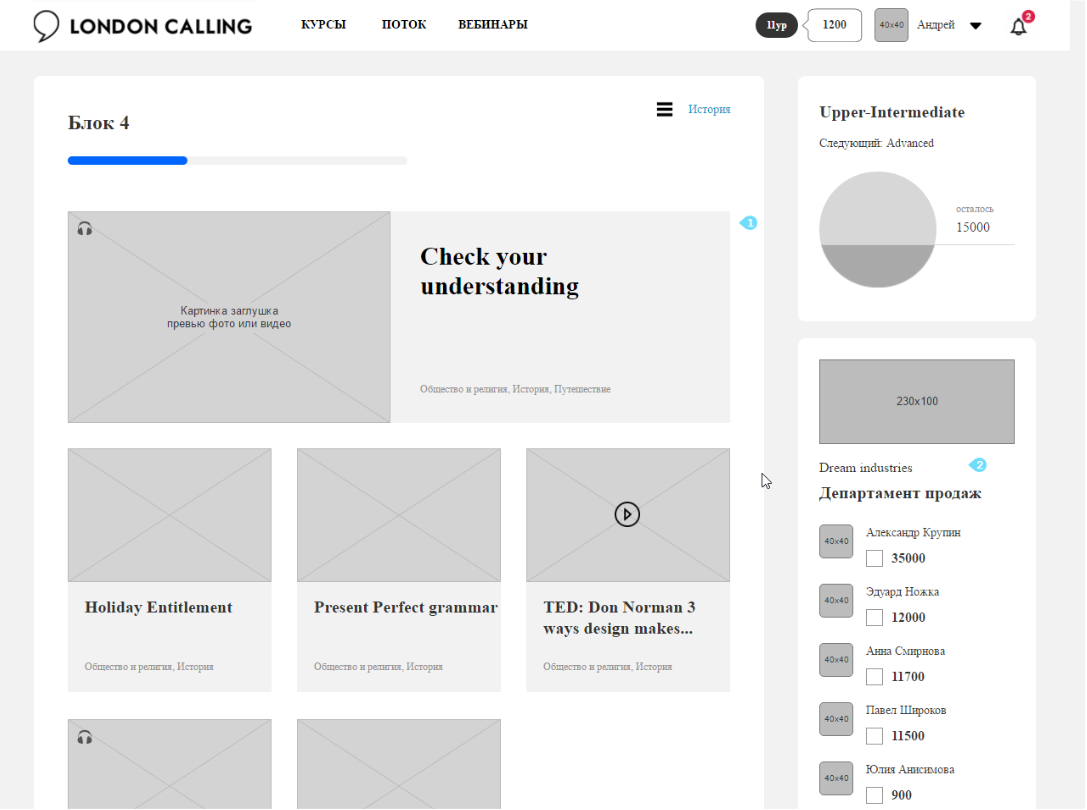
\includegraphics[width=0.8\textwidth]{languageServiceWireframe.png}
\end{center}

Рисуют такие вещи с помощью специальных инструментов:

\begin{itemize}
    \item Balsamiq~--- один из самых старых, простых и примитивных, к тому же десктопный (хотя относительно недавно научился и в веб).
    \item Ninjamock~--- то же самое, что Balsamiq, только посовременнее, изначально в вебе и для коллаборативной разработки, имеет бесплатный план (и не очень дорогой платный, при этом по сей день дружественен к пользователям из России).
    \item Axure~--- мощная крутая штука, выбор профессионала.
\end{itemize}

\subsection{Дизайн-макет (цифровой mockup)}

Дизайн-макет или мокап создаётся дизайнером на основе wireframe. Основное его отличие от wireframe~--- большая похожесть на конечное решение. То есть в инструментах, которые для создания мокапов используются, часто пользуются библиотеками элементов управления, специфичных для конечной платформы (всякие мобильные контролы по гайдлайнам Android, iOS и т.п.). Часто мокапы делаются pixel-perfect, то есть задача разработчика потом просто в точности повторить этот дизайн в коде. Более того, всякие модные современные инструменты для прототипирования сайтов могут сами предоставлять html- и css-код , реализующий отдельные компоненты макета.

Так, wireframe выше в дизайн-макете выглядел как-то так:

\begin{center}
    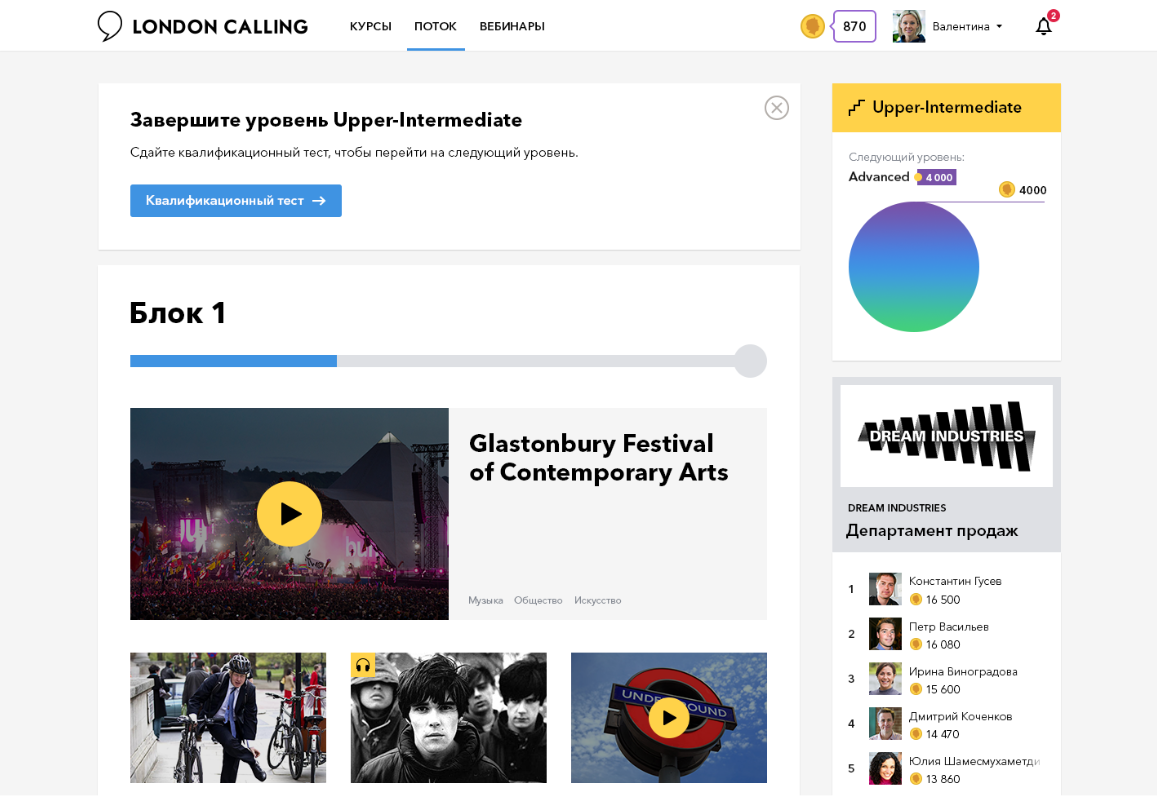
\includegraphics[width=0.8\textwidth]{designLayout.png}
\end{center}

К слову, это как раз тот случай, когда при реализации практически один-в-один был воплощён в жизнь разработанный дизайн-макет.

Такие вещи тоже рисуются в специальных инструментах:

\begin{itemize}
    \item UXPin~---  типа Axure, только можно делать прототипы более задизайненные.
    \item Sketch~--- красивый и удобный (стандарт де-факто в рисовании дизайн-макетов), но только под Mac. Импорт его формата есть почти во всех остальных инструментов.
    \item Invision app~--- интерактивность, поддержка юзабилити-тестирования, поддержка мобильных прототипов. По мнению коллег, занимающихся UX профессионально, самый крутой инструмент сейчас для дизайн-макетов.
\end{itemize}

\subsection{Интерактивный прототип}

То же самое, что макеты и мокапы выше, но интерактивные. Можно использовать в тестировании на пользователях, показывать заказчику, использовать как средство коммуникации между дизайнерами и разработчиками.

Самый простой пример интерактивного прототипа мобильного приложения~--- сделать PDF с кнопками, открывающими другие страницы, и открыть её на телефоне в полноэкранном режиме. Впрочем, многие существующие инструменты умеют это делать более интеллектуально. 

Инструменты:

\begin{itemize}
    \item Principle~--- удобный и крутой, но только под мак;
    \item Marvel~--- по функциональности по сути то же самое;
    \item Proto.io~--- для мобильных прототипов.
\end{itemize}

\subsection{Прототипирование кодом}

Отдельный подход, сильно на любителя. Занимает больше времени, зато вроде как получается полу-рабочее полу-приложение. Как MVP для стартапа, может, и подойдёт, но вообще так мало кто делает. 

Инструменты:

\begin{itemize}
    \item Macaw;
    \item Framer.
\end{itemize}

Впрочем, такой подход часто применяется при разработке уже настоящего прототипа, благо современный инструментарий разработки пользовательских интерфейсов <<полноценных>> технологий разработки приложений вполне позволяет делать <<живые>> прототипы. Например, язык XAML в библиотеке WPF для .NET позволяет делать хоть полноценные приложения в декларативном стиле, без строчки кода, прототипы UX-то уж тем более.

\subsection{Немного статистики}

Ну и в завершении~--- картинка с результатами опроса 86 UX-дизайнеров по тому, какие артефакты они создают в своих проектах\footnote{Более детально можно посмотреть тут: \url{https://www.nngroup.com/articles/common-ux-deliverables/} (дата обращения: 12.03.2023).}.

\begin{center}
    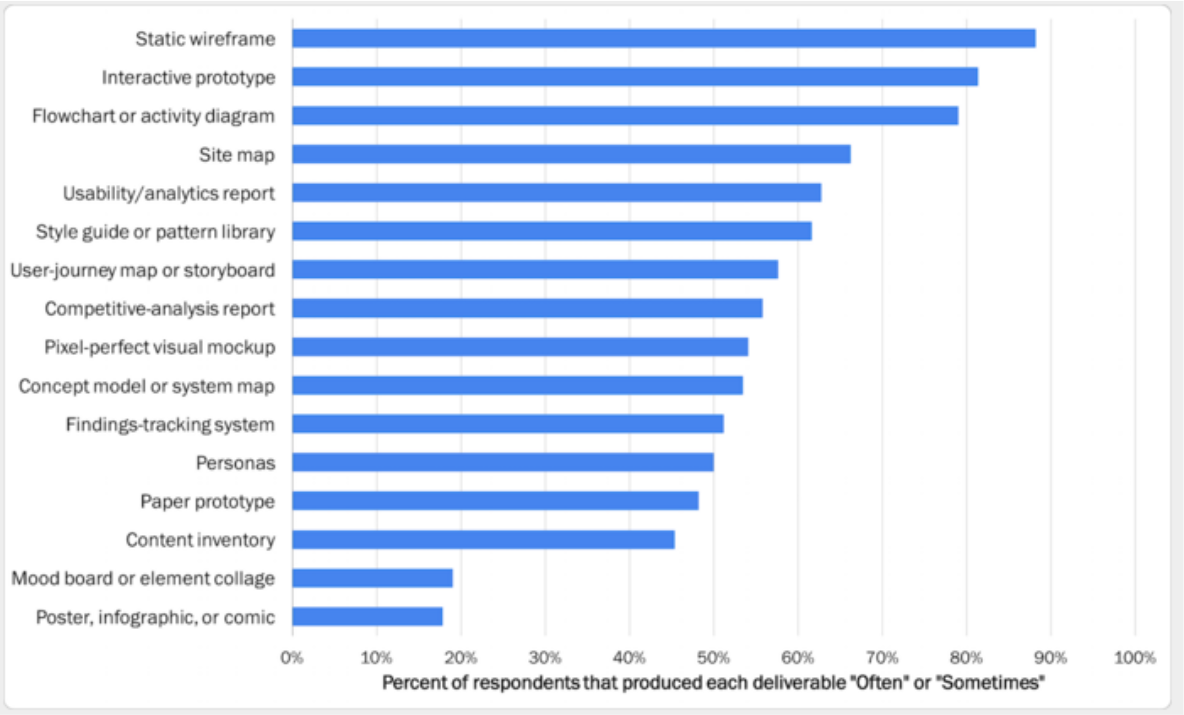
\includegraphics[width=0.7\textwidth]{statistics.png}
\end{center}

\section{Исследования продукта}

Ну и если уже есть какой-то прототип или проводится редизайн или переработка существующего продукта, его можно и нужно анализировать. Для этого применяются следующие практики:

\begin{itemize}
    \item Аудит продукта/прототипа или конкурентов
    \item Экспертная оценка интерфейса
    \item Качественный анализ пользователей (интервью)
    \item Полевое наблюдение (открытое и скрытое)
    \item Анализ данных
    \begin{itemize}
        \item Статистика использования
        \item Выполнение сценариев
        \item Количественный анализ пользователей
    \end{itemize}
    \item A/B-тестирование\footnote{\url{http://texterra.ru/blog/kak-provodit-a-b-testiro>vanie.html} (дата обращения: 12.03.2023).}
    \item Эвристический анализ интерфейса\footnote{\url{https://turumburum.ua/blog/evristicheskaya-otsenka-yuzabiliti-sayta} (дата обращения: 12.03.2023).}
    \item Usability-исследование\footnote{\url{https://ru.wikipedia.org/wiki/Юзабилити-тестирование} (дата обращения: 12.03.2023).}
    \begin{itemize}
        \item Фокус-группа
        \item Опросники
        \item Eye tracking
    \end{itemize}
\end{itemize}

\section{Полезные ссылки}

The UX Design Process: An Actionable Guide To Your First Job In UX: \url{https://careerfoundry.com/en/blog/ux-design/the-ux-design-process-an-actionable-guide-to-your-first-job-in-ux/} (дата обращения: 12.03.2023).

\end{document}
